% The Clever Algorithms Project: http://www.CleverAlgorithms.com
% (c) Copyright 2011 Jason Brownlee. Some Rights Reserved. 
% This work is licensed under a Creative Commons Attribution-Noncommercial-Share Alike 2.5 Australia License.

% This is a chapter

\renewcommand{\bibsection}{\subsection{\bibname}}
\begin{bibunit}

\chapter{Optimization}
\label{ch:optimization}
\index{Optimization}

\section{Overview}
This chapter describes unconstrained Optimization methods that common in the field of Machine Learning.

% Types of Optimization Algorithms
\subsection{Taxonomy}
\index{Direct Search}
\index{Stochastic Direct Search}
\index{Convex Optimization}
\index{Nonlinear Optimization}
The field of function optimization is mature, traditionally referred to as Mathematical Programming. Optimization forms the core of most Machine Learning methods, and many explicitly use a classical optimization method. For the purposes of our understanding of optimization in the context of Machine Learning, we can consider the following types of optimization algorithms:

\begin{itemize}
	\item \textbf{Direct Search}: These are methods that only sample the function to decide how to progress the search. These are generally inefficient compared to derivative based approaches, but have the advantage of working on functions where a derivative cannot be computed or cannot be computed easily, such as noisy or discontinuous functions. Any gradient information is inferred from direct samples. The name `Direct Search' was proposed by Hooke and Jeeves \cite{Hooke1961} and a modern review of such methods can be seen in Lewis et~al. \cite{Lewis2000}. Examples of Direct Search algorithms include Line Search methods, Pattern Search, Rosenbrock's Method, Nelder-Mead Search, and Powell's Conjugate Direction Method.

	\item \textbf{Stochastic Direct Search}: These are methods that are stochastic processes that sample the objective function in a direct manner. Examples include Simulated Annealing, Genetic Algorithms, and Particle Swarm Optimization.

	\item \textbf{First-order Derivative}: These are methods that require the calculation of the first partial derivative (function gradient) of the objective function that is being optimized. For those problems where a gradient can be computed directly, these methods are generally more efficient (converge faster) than Direct Search methods. Examples include Gradient Descent, Steepest Descent, and Conjugate Gradient Descent.

	\item \textbf{Second-order Derivative}: These are methods that require the calculation of a Hessian matrix of second partial derivatives (or an approximation thereof) in addition to the first-order gradient. Some second-order methods also require the storage of a matrix which must be maintained during the search procedure. Compared to first-order methods, these methods have a grater computational and/or memory expense although are generally more efficient (converge faster) given the grater amount of information available about the function. Examples include Newton's Method (Newton-Raphson Method), Gauss-Newton Method, Levenberg-Marquardt Method, and quasi-Newton Methods (Hessian approximation methods) such as BFGS, DFP Method, Broyden's method and the SR1 Method.
\end{itemize}

% Nomenclature
\subsection{Nomenclature}
% conceputlaization
Function optimization is commonly conceptualized geometrically, where the parameters of the function define an $n$-dimensional search space and the role of the algorithm is to locate the desired point within that search space.

% optima
A problem may be referred to as an objective function, cost function, utility function, or loss function and it may be minimization or maximization. One may talk about the objective of the function in the abstract as a function extremum or function optimum. 
% shape
A function have one or more optima, and the shape of the functions response surface (the result of the function given parameter values) is referred to as being unimodal or multimodal respectively. The single optimum of a unimodal function means that the local optimum is the global optimum. Highly-nonlinear and multimodal problems can have many optima, meaning that some optimization methods can get caught in a local optimum and fail to fund the global optimum.

% convex
Many Machine Learning methods have been defined with the optimization of a convex function as the core problem. For our purposes, a convex function is unimodal and is a type of function that looks like a bowl or basin shape when in two-dimensions.

% references
\subsection{Further Reading}
% general
There are many texts on modern optimization methods. Some good general reference texts include Boyd and Vandenberghe  who provide a comprehensive introduction into the field of convex function optimization \cite{Boyd2004}, and Griva et~al. who provide a broader walk of the field of linear and non-linear optimization \cite{Griva2009}. Nocedal and Wright also provide a thorough text on numerical optimization methods \cite{Nocedal1999}.
% for machine learning
Reed et~al. provide an excellent overview of modern optimization methods in the context of their adaptation for use in Artificial Neural Networks \cite{Reed1998} (Chapter 10).
% R 
Braun et~al. provide a gentle introduction to optimization algorithms in R with some worked examples \cite{Braun2007} (Chapter 7).

\putbib
\end{bibunit}

\newpage\begin{bibunit}% The Clever Algorithms Project: http://www.CleverAlgorithms.com
% (c) Copyright 2011 Jason Brownlee. Some Rights Reserved. 
% This work is licensed under a Creative Commons Attribution-Noncommercial-Share Alike 2.5 Australia License.

% Name
% The algorithm name defines the canonical name used to refer to the technique, in addition to common aliases, abbreviations, and acronyms. The name is used in terms of the heading and sub-headings of an algorithm description.
\section{Golden Section Search} 
\label{sec:golden_section_search}
\index{Golden Section Search}
\index{Golden Mean Search}

% other names
% What is the canonical name and common aliases for a technique?
% What are the common abbreviations and acronyms for a technique?
\emph{Golden Section Search, Golden Mean Search.}

% Taxonomy: Lineage and locality
\subsection{Taxonomy}
\index{Line Search}
\index{Direct Search}
\index{Pattern Search}
\index{Brent's Method}
% To what fields of study does a technique belong?
Golden Section Search is a Line Search method for Global Optimization in one-dimension. It is a Direct Search (Pattern Search) method as it samples the function to approximate a derivative rather than computing it directly.
% What are the closely related approaches to a technique? 
The Golden Section Search is related to pattern searches of discrete ordered lists such as the Binary Search and the  Fibonacci Search. It is related to other Line Search algorithms such as Brent's Method and more generally to other direct search optimization methods such as the Nelder-Mead Method.

% Strategy: Problem solving plan
% The strategy is an abstract description of the computational model. The strategy describes the information processing actions a technique shall take in order to achieve an objective. The strategy provides a logical separation between a computational realization (procedure) and a analogous system (metaphor). A given problem solving strategy may be realized as one of a number specific algorithms or problem solving systems. The strategy description is textual using information processing and algorithmic terminology.
\subsection{Strategy}
% What is the information processing objective of a technique?
The information processing objective of the method is to locate the extremum of a function.
% What is a techniques plan of action?
It does this by directly sampling the function using a pattern of three points. The points form the brackets on the search: the first and the last points are the current bounds of the search, and the third point partitions the intervening space. The partitioning point is selected so that the ratio between the larger partition and the whole interval is the same as the ratio of the larger partition to the small partition, known as the golden ratio ($\phi$). The partitions are compared based on their function evaluation and the better performing section is selected as the new bounds on the search. The process recurses until the desired level of precision (bracketing of the optimum) is obtained or the search stalls.

% Heuristics: Usage guidelines
% The heuristics element describe the commonsense, best practice, and demonstrated rules for applying and configuring a parameterized algorithm. The heuristics relate to the technical details of the techniques procedure and data structures for general classes of application (neither specific implementations not specific problem instances). The heuristics are described textually, such as a series of guidelines in a bullet-point structure.
\subsection{Heuristics}
% What are the suggested configurations for a technique?
% What are the guidelines for the application of a technique to a problem instance?

\begin{itemize}
	\item Assumes that the function is convex and unimodal specifically, that the function has a single optimum and that it lies between the bracketing points.
	\item Intended to find the extrema one-dimensional continuous functions.
	\item It was shown to be more efficient than an equal-sized partition line search.
	\item The termination criteria is a specification on the minimum distance between the brackets on the optimum.
	\item It can quickly locate the bracketed area of the optimum but is less efficient at locating the specific optimum.
	\item Once a solution of desired precision is located, it can be provided as the basis to a second search algorithm that has a faster rate of convergence.
\end{itemize}

% sample script in R
\subsection{Code Listing}
\index{Parabolic Interpolation}
% listing
Listing~\ref{stats_golden_section_search} provides a code listing Golden Section Search method in R solving a one-dimensional nonlinear unconstrained optimization function. Figure~\ref{plot:golden_section_search_result} provides a plot of the test problem with the located minimum highlighted.

% algorithm and package
The example uses the \texttt{optimize()} function in the \texttt{stats} core package \cite{RDCT2011a}. This function uses a Golden Section Search with successive Parabolic Interpolation. This combination of a Line Search followed successively by Parabolic Interpolation is a common pattern for improving the overall result by leveraging the non-parametric nature of the former and the speed of convergence of the latter methods. The \texttt{optimize()} function is for One-Dimensional Optimization. For more information on this library type: \texttt{library(help="stats")}, and for more information on the function type: \texttt{?optimize}.

% problem
The test problem is the basin function in one-dimension where the optimum is at $f(0)=0$ and the domain is defined as $x \in [-5,5]$. 

\lstinputlisting[firstline=7,language=r,caption={Example of Golden Section Search in R using the \texttt{optimize()} function in the \texttt{stats} core package.}, label=stats_golden_section_search]{../src/algorithms/optimization/stats_golden_section_search.R}

\begin{figure}[htp]
\centering
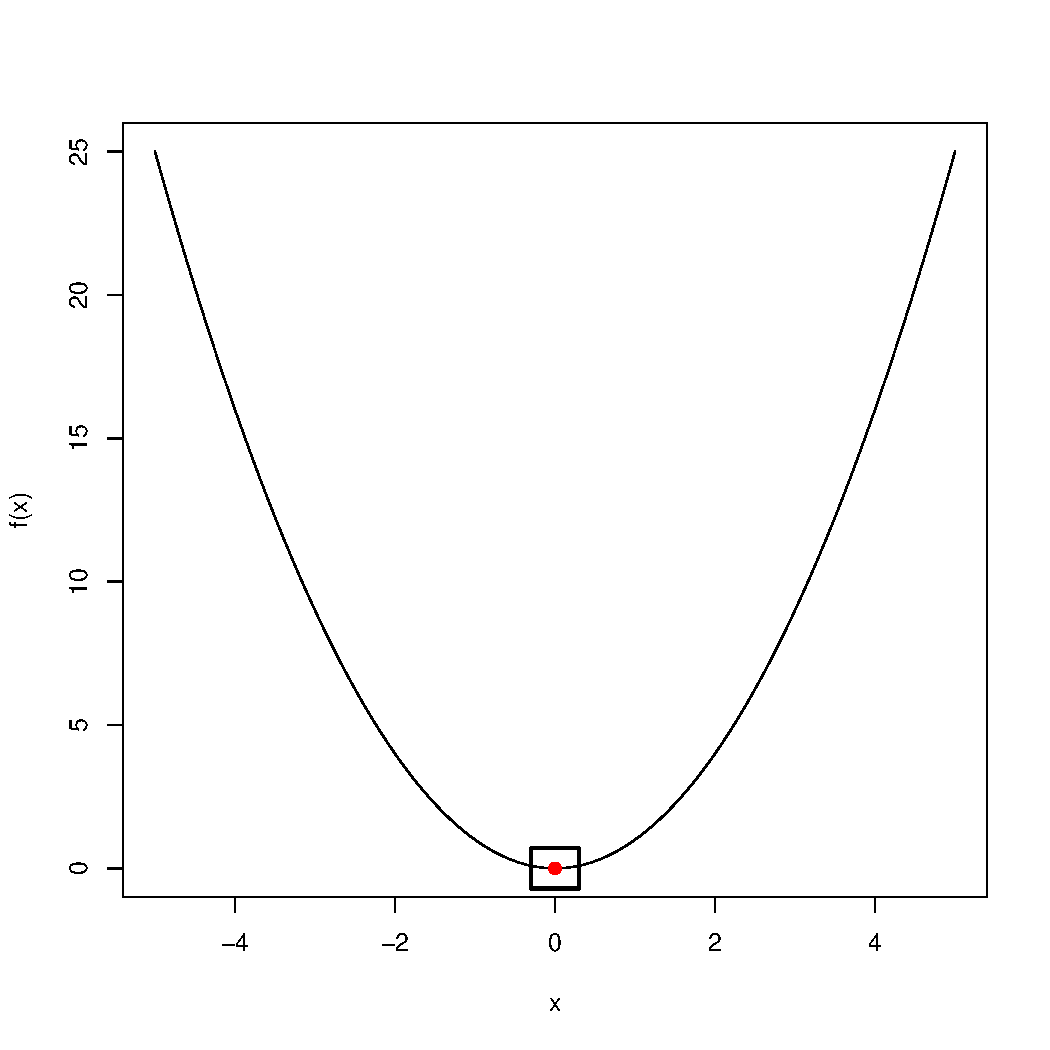
\includegraphics[scale=0.45]{a_optimization/golden_section_search_result.pdf}
\caption{Plot of the basin function in one-dimension with the located minimum highlighted.}
\label{plot:golden_section_search_result}
\end{figure}

The \texttt{stats} core package also provides an implementation of Brent's method in the \texttt{optim} function.

% References: Deeper understanding
% The references element description includes a listing of both primary sources of information about the technique as well as useful introductory sources for novices to gain a deeper understanding of the theory and application of the technique. The description consists of hand-selected reference material including books, peer reviewed conference papers, journal articles, and potentially websites. A bullet-pointed structure is suggested.
\subsection{References}
% What are the primary sources for a technique?
% What are the suggested reference sources for learning more about a technique?

% primary sources
\subsubsection{Primary Sources}
% seminal
The method was described by Kiefer in 1953 as a method for finding the maximum of a function without regularity conditions such as continuity and function derivatives \cite{Kiefer1953}.
Johnson provided an early description of the method in a technical report for RAND Corporation \cite{Johnson1955}.

% more info
\subsubsection{More Information}
% useful
Press et~al.\ provide a terse and practical introduction to the method with well-commented sample code in the C programming language \cite{Press2007}.
% early
Brent provides an early treatment of the method is his text on minimization without derivatives \cite{Brent1973}.
% text books
Many text books on scientific computing or numerical analysis include a section on Golden Section Search, for example see Heath \cite{Heath2002}.

% END
\putbib\end{bibunit}
\newpage\begin{bibunit}% The Clever Algorithms Project: http://www.CleverAlgorithms.com
% (c) Copyright 2011 Jason Brownlee. Some Rights Reserved. 
% This work is licensed under a Creative Commons Attribution-Noncommercial-Share Alike 2.5 Australia License.

% Name
% The algorithm name defines the canonical name used to refer to the technique, in addition to common aliases, abbreviations, and acronyms. The name is used in terms of the heading and sub-headings of an algorithm description.
\section{Nelder-Mead Method} 
\label{sec:neldermead}
\index{Nelder-Mead Method}
\index{Simplex Algorithm}
\index{Amoeba Algorithm}

% other names
% What is the canonical name and common aliases for a technique?
% What are the common abbreviations and acronyms for a technique?
\emph{Nelder-Mead Method, Downhill Simplex Method, Simplex Method, Amoeba Algorithm.}

% Taxonomy: Lineage and locality
\subsection{Taxonomy}
% To what fields of study does a technique belong?
The Nelder-Mead Method is an optimization algorithm for multidimensional nonlinear unconstrained functions.
It is a Direct Search Method in that it does not use a function gradient during the procedure. It is a Pattern Search in that it uses a geometric pattern to explore the problem space.
% What are the closely related approaches to a technique?
It is related to other Direct Search optimization methods such as Hooke and Jeeves' Pattern Search that also uses a geometric pattern to optimize an objective function.

% Strategy: Problem solving plan
% The strategy is an abstract description of the computational model. The strategy describes the information processing actions a technique shall take in order to achieve an objective. The strategy provides a logical separation between a computational realization (procedure) and a analogous system (metaphor). A given problem solving strategy may be realized as one of a number specific algorithms or problem solving systems. The strategy description is textual using information processing and algorithmic terminology.
\subsection{Strategy}
% What is the information processing objective of a technique?
The information processing objective of the Nelder-Mead Method is to locate the extremum of a function.
% What is a techniques plan of action?
This is achieved by overlaying a simplex (geometrical pattern) in the domain and iteratively increasing and/or reducing its size until an optimal value is found. The simplex is defined always with $n+1$ vertices, where $n$ is the number of dimensions of the search space (i.e. a triangle for a 2D problem).

The process involves identifying the worst performing point of the complex and replacing it with a point reflected through the centroid (center point) of the remaining points. The simplex can be deformed (adapt itself to the topology of the search space) by expanding away from the worst point, contract along one dimension away from the worst point, or contract on all dimensions towards the best point.

% Heuristics: Usage guidelines
% The heuristics element describe the commonsense, best practice, and demonstrated rules for applying and configuring a parameterized algorithm. The heuristics relate to the technical details of the techniques procedure and data structures for general classes of application (neither specific implementations not specific problem instances). The heuristics are described textually, such as a series of guidelines in a bullet-point structure.
\subsection{Heuristics}
% What are the suggested configurations for a technique?
% What are the guidelines for the application of a technique to a problem instance?

\begin{itemize}
	\item It can be used with multi-dimensional functions (one or more parameters) and with non-linear response surfaces.
	\item It does not use a function derivative meaning that it can be used on non-differentiable functions, discontinuous functions, non-smooth functions, and noisy functions.
	\item As a direct search method it is consider inefficient and slow relative to modern derivative-based methods.
	\item It is dependent on the starting position and can be caught by local optimum in multimodal functions.
	\item The stopping criteria can be a minimum change in the best position. 
	\item The nature of the simplex structure can mean it can get stuck in non-optimal areas of the search space, this is more likely if the size of the initial simplex is too large.
	\item When the method does work (is appropriate for the function being optimized) it has been shown to be fast and robust.
\end{itemize}

% sample script in R
\subsection{Code Listing}
% listing
Listing~\ref{stats_nelder_mead} provides a code listing of the Nelder-Mead method in R solving a two-dimensional nonlinear optimization function. Figure~\ref{plot:nelder_mead_result} provides a plot of the test problem with the located minimum highlighted.

% algorithm and package
The example uses the \texttt{optim()} function in the \texttt{stats} core package configured to use the ``Nelder-Mead'' method \cite{RDevelopmentCoreTeam2011a}. The example uses the algorithm default parameters of $\alpha=1.0$ (reflection factor), $\beta=0.5$ (contraction factor), and $\gamma=2.0$ (expansion factor). The procedure will stop if there is no improvement from an iteration (change in response is less than the square root of the machines precision). The \texttt{optim()} function is for General-purpose Optimization, for more information on this library type: \texttt{library(help="stats")}, and for more information on the function type: \texttt{?optim}.

% problem
The test problem is the Rosenbrock function in two-dimensions where the optimum is at $x,y=1$. The starting position for the algorithm is taken as a random point $x,y \in [-3,3]$.

\lstinputlisting[firstline=7,language=r,caption={Example of Nelder-Mead in R using the \texttt{optim()} function in the \texttt{stats} core package.}, label=stats_nelder_mead]{../src/algorithms/optimization/stats_nelder_mead.R}

\begin{figure}[htp]
\centering
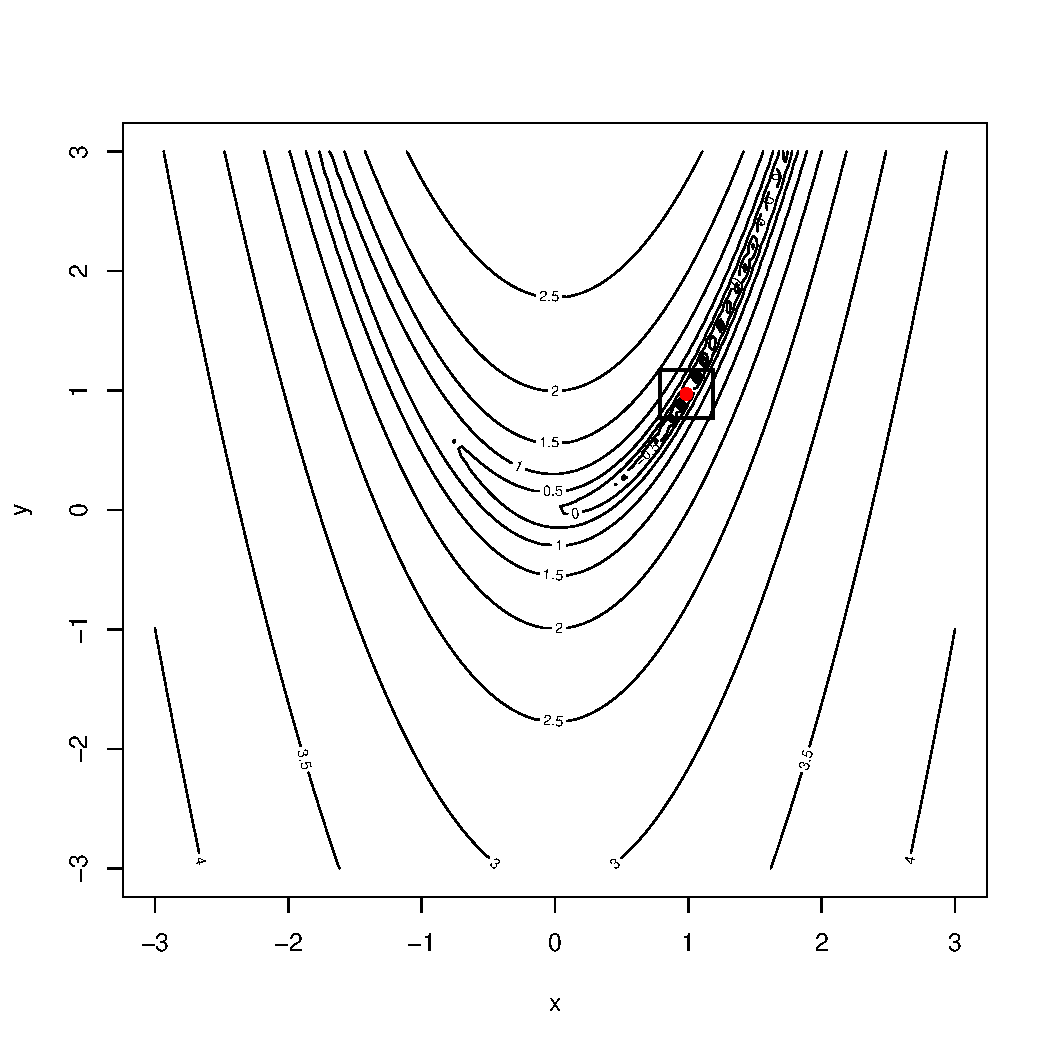
\includegraphics[scale=0.45]{a_optimization/nelder_mead_result.pdf}
\caption{Contour plot of the Rosenbrock function with the located minimum highlighted.}
\label{plot:nelder_mead_result}
\end{figure}

% other packages
The \texttt{gsl} package in the \texttt{multimin()} function provides an implementation of Nelder-Mead algorithm that makes use of the GNU Scientific Library \cite{Hankin2011}.
The \texttt{neldermead} package also provides an implementation of the algorithm \cite{Bihorel2011}.

% References: Deeper understanding
% The references element description includes a listing of both primary sources of information about the technique as well as useful introductory sources for novices to gain a deeper understanding of the theory and application of the technique. The description consists of hand-selected reference material including books, peer reviewed conference papers, journal articles, and potentially websites. A bullet-pointed structure is suggested.
\subsection{References}
% What are the primary sources for a technique?
% What are the suggested reference sources for learning more about a technique?

% primary sources
\subsubsection{Primary Sources}
% seminal
The Simplex optimization algorithm was proposed by Spendley et~al.\ in 1962 that used a simplex and a reflection operator to replace the worst point of the structure \cite{Spendley1962}.
Nelder and Mead extended the method by adding the expansion and contraction rules to the process to increase the rate of convergence in what became known as the Nelder-Mead method \cite{Nelder1965}.

% more info
\subsubsection{More Information}
% study
Lagarias et~al.\ provide a comment of the convergence properties of the Nelder-Mead method on convex one- and two-dimensional problems as well as a careful and complete description of the method clearing up some ambiguous points on its original implementation \cite{Lagarias1998}. Press et~al.\ provide a good summary of the method with sample code in the C programming language \cite{Press2007}. Lewis et~al.\ provide an overview of the procedure and a contemporary perspective on its capabilities in the context of other Direct Search methods \cite{Lewis2000}.
% book
Walters provides a book that focuses on the method which he refers to as Sequential Simplex Optimization \cite{Walters1991}.

% END
\putbib\end{bibunit}
\newpage\begin{bibunit}% The Clever Algorithms Project: http://www.CleverAlgorithms.com
% (c) Copyright 2013 Jason Brownlee. Some Rights Reserved. 
% This work is licensed under a Creative Commons Attribution-Noncommercial-Share Alike 2.5 Australia License.


% Name
% The algorithm name defines the canonical name used to refer to the technique, in addition to common aliases, abbreviations, and acronyms. The name is used in terms of the heading and sub-headings of an algorithm description.
\section{Gradient Descent} 
\label{sec:gradient_descent}
\index{Gradient Descent}
\index{Gradient Ascent}

% other names
% What is the canonical name and common aliases for a technique?
% What are the common abbreviations and acronyms for a technique?
\emph{Gradient Descent, Gradient Ascent.}

% Taxonomy: Lineage and locality
\subsection{Taxonomy}
\index{Steepest Descent Method}
\index{Stochastic Gradient Descent}
\index{Online Gradient Descent}
\index{Batch Gradient Descent}
% To what fields of study does a technique belong?
Gradient Descent is a first-order derivative optimization method for unconstrained nonlinear function optimization. It is called Gradient Descent because it was envisioned for function minimization. When applied to function maximization it may be referred to as Gradient Ascent. 

% What are the closely related approaches to a technique? 
Steepest Descent Search is an extension that performs a Line Search on the line of the gradient to the locate the optimum neighboring point (optimum step or steepest step).
Batch Gradient Descent is an extension where the cost function and its derivative are computed as the summed error on a collection of training examples.
Stochastic Gradient Descent (or Online Gradient Descent) is like Batch Gradient Descent except that the cost function and derivative are computed for each training example.

% Strategy: Problem solving plan
% The strategy is an abstract description of the computational model. The strategy describes the information processing actions a technique shall take in order to achieve an objective. The strategy provides a logical separation between a computational realization (procedure) and a analogous system (metaphor). A given problem solving strategy may be realized as one of a number specific algorithms or problem solving systems. The strategy description is textual using information processing and algorithmic terminology.
\subsection{Strategy}
% What is the information processing objective of a technique?
The information processing objective of the method is to locate the extremum of a function.
% What is a techniques plan of action?
This is achieved by first selecting a starting point in the search space. For a given point in the search space, the derivative of the cost function is calculated and a new point is selected down the gradient of the functions derivative at a distance of $\alpha$ (the step size parameter) from the current point. 

% Heuristics: Usage guidelines
% The heuristics element describe the commonsense, best practice, and demonstrated rules for applying and configuring a parameterized algorithm. The heuristics relate to the technical details of the techniques procedure and data structures for general classes of application (neither specific implementations not specific problem instances). The heuristics are described textually, such as a series of guidelines in a bullet-point structure.
\subsection{Heuristics}
% What are the suggested configurations for a technique?
% What are the guidelines for the application of a technique to a problem instance?

\begin{itemize}
	\item The method is limited to finding the local optimum, which if the function is convex, is also the global optimum.
	\item It is considered inefficient and slow (linear) to converge relative to modern methods. Convergence can be slow if the gradient at the optimum flattens out (gradient goes to 0 slowly). Convergence can also be slow if the Hessian is poorly conditioned (gradient changes rapidly in some directions and slower in others).
	\item The step size ($\alpha$) may be constant, may adapt with the search, and may be maintained holistically or for each dimension.
	\item The method is sensitive to initial conditions, and as such, it can be common to repeat the search process a number of times with randomly selected initial positions.
	\item If the step size parameter ($\alpha$) is too small, the search will generally take a large number of iterations to converge, if the parameter is too large can overshoot the function's optimum.
	\item Compared to non-iterative function optimization methods, gradient descent has some relative efficiencies when it comes to scaling with the number of features (dimensions).
\end{itemize}

% sample script in R
\subsection{Code Listing}
% listing
Listing~\ref{gradient_descent} provides a code listing Gradient Descent algorithm in R solving a two-dimensional nonlinear optimization function. Figure~\ref{plot:gradient_descent_result} provides a plot of the test problem with the located minimum highlighted.

% algorithm and package
The example provides a custom written \texttt{gradient\_descent()} function for locating the minimum of a two-dimensional function.
% problem
The test problem is the basin function in two-dimensions where the optimum is at $f(0)=0$ and the domain is defined as $x \in [-3,3]$. 

\lstinputlisting[firstline=7,language=r,caption={Example of Gradient Descent in R using a custom function.}, label=gradient_descent]{../src/algorithms/optimization/gradient_descent.R}

\begin{figure}[htp]
\centering
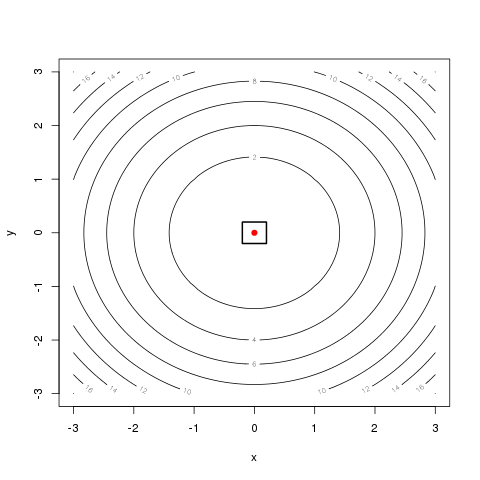
\includegraphics[scale=0.45]{a_optimization/gradient_descent_result.png}
\caption{Contour plot of the basin function with the located minimum highlighted.}
\label{plot:gradient_descent_result}
\end{figure}

% other packages
Another other packages that provides an implementation of Gradient Descent include \texttt{animation}. The \texttt{gsl} package in the \texttt{multimin()} function provides an implementation of Steepest Descent that makes use of the GNU Scientific Library \cite{Hankin2011}.

% References: Deeper understanding
% The references element description includes a listing of both primary sources of information about the technique as well as useful introductory sources for novices to gain a deeper understanding of the theory and application of the technique. The description consists of hand-selected reference material including books, peer reviewed conference papers, journal articles, and potentially websites. A bullet-pointed structure is suggested.
\subsection{References}
% What are the primary sources for a technique?
% What are the suggested reference sources for learning more about a technique?

% primary sources
\subsubsection{Primary Sources}
% seminal
The method of Steepest Descent can be traced back to Cauchy in 1847 who proposed the use of the gradient to minimize a system of simultaneous equations \cite{Cauchy1847} (French). Gradient Descent may be considered a relaxation of this original method.
% early extensions
There have been many extensions of the method. Curry provides an early extension that seeks the first stable point on the line following the gradient \cite{Curry1944}. Spang provided a good early review of minimization methods providing context for Steepest Descent \cite{Spang1962}.

% more info
\subsubsection{More Information}
Gradient Descent is a cornerstone of Machine Learning methods and is the go-to method for optimizing the cost or loss functions at the core of many modern algorithms. As such, a description can be found in any good text on Artificial Intelligence, Machine Learning, or Numerical Methods.


% END
\putbib\end{bibunit}
\newpage\begin{bibunit}% The Clever Algorithms Project: http://www.CleverAlgorithms.com
% (c) Copyright 2011 Jason Brownlee. Some Rights Reserved. 
% This work is licensed under a Creative Commons Attribution-Noncommercial-Share Alike 2.5 Australia License.

% Name
% The algorithm name defines the canonical name used to refer to the technique, in addition to common aliases, abbreviations, and acronyms. The name is used in terms of the heading and sub-headings of an algorithm description.
\section{Conjugate Gradient Method} 
\label{sec:conjugate_gradient}
\index{Conjugate Gradient Method}
\index{Nonlinear Conjugate Gradient Method}

% other names
% What is the canonical name and common aliases for a technique?
% What are the common abbreviations and acronyms for a technique?
\emph{Conjugate Gradient Method, Nonlinear Conjugate Gradient Method.}

% Taxonomy: Lineage and locality
\subsection{Taxonomy}
% To what fields of study does a technique belong?
Conjugate Gradient Method is a first-order derivative optimization method for multidimensional nonlinear unconstrained functions.
% What are the closely related approaches to a technique?
It is related to other first-order derivative optimization algorithms such as Gradient Descent and Steepest Descent.

% Strategy: Problem solving plan
% The strategy is an abstract description of the computational model. The strategy describes the information processing actions a technique shall take in order to achieve an objective. The strategy provides a logical separation between a computational realization (procedure) and a analogous system (metaphor). A given problem solving strategy may be realized as one of a number specific algorithms or problem solving systems. The strategy description is textual using information processing and algorithmic terminology.
\subsection{Strategy}
% What is the information processing objective of a technique?
The information processing objective of the technique is to locate the extremum of a function.
% What is a techniques plan of action?
From a starting position, the method first computes the gradient to locate the direction of steepest descent, then performs a line search to locate the optimum step size ($\alpha$). The method then repeats the process of computing the steepest direction, computes direction of the search, and performing a line search to locate the optimum step size. A parameter $\beta$ defines the direction update rule based on the gradient and can be computed using one of a number of methods.
% difference from steepest descent
The difference between Conjugate Gradient and Steepest Descent is that it uses conjugate directions rather than local gradients to move downhill towards the function minimum, which can be very efficient.

% Heuristics: Usage guidelines
% The heuristics element describe the commonsense, best practice, and demonstrated rules for applying and configuring a parameterized algorithm. The heuristics relate to the technical details of the techniques procedure and data structures for general classes of application (neither specific implementations not specific problem instances). The heuristics are described textually, such as a series of guidelines in a bullet-point structure.
\subsection{Heuristics}
% What are the suggested configurations for a technique?
% What are the guidelines for the application of a technique to a problem instance?

\begin{itemize}
	\item It is more efficient than Steepest Descent, for example it may take a straight line path down narrow valley's, whereas Steepest Descent would have to zig-zag (pinball) down the valley.
	\item Devolves into Steepest Descent if the conjugate direction is reset each iteration.
	\item It is almost as fast as second-order gradient methods, requiring just $n$ iterations to locate an optimum for suitable functions (where $n$ is the number of parameters).
	\item It does not maintain a Hessian matrix (like BFGS) and therefore may be suitable for larger problems with many variables.
	\item The method is most efficient (works the best) with quadratic or quadratic-like functions, or where the function is approximately quadratic near the optimum.
	\item The method is sensitive to its starting position on non-convex problems.
	\item The learning rate (step size $\alpha$) does not have to be specified as a line search is used to locate the optimum value as needed.
	\item Common methods for computing the direction update rule ($\beta$) are the Hestenes-Stiefel \cite{Hestenes1952}, Fletcher-Reeves \cite{Fletcher1964}, Polak-Ribi\`ere \cite{Polak1969} (French), and Beale-Sorenson \cite{Beale1972, Sorenson1969} methods. The Polak-Ribi\`ere method generally works better in practice for non-quadratic functions.
	\item It is dependent on the accuracy of the line search, errors introduced both from this and the less-than quadratic nature of the response surface will result in more frequent updates to the direction and a less efficient search.
	\item To avoid the search degenerating, consider restarting the search process after $n$ iterations, where $n$ is the number of function parameters.
\end{itemize}


% sample script in R
\subsection{Code Listing}
% listing
Listing~\ref{stats_conjugate_gradient} provides a code listing of the Conjugate Gradient method in R solving a two-dimensional nonlinear optimization function. Figure~\ref{plot:conjugate_gradient_result} provides a plot of the test problem with the located minimum highlighted.

% algorithm and package
The example uses the \texttt{optim()} function in the \texttt{stats} core package configured to use the Conjugate Gradient Method as ``CG'' \cite{RDCT2011a}. The method supports three update methods: Fletcher-Reeves update (default), Polak-Ribi\`ere update, and the Beale-Sorenson update. The \texttt{optim} function is for General-purpose Optimization, for more information on this library type: \texttt{library(help="stats")}, and for more information on the function type: \texttt{?optim}.

% problem
The test problem is the Rosenbrock function in two-dimensions where the optimum is at $x,y=1$. The starting position for the algorithm is taken as a random point $x,y \in [-3,3]$. The gradient for this function is specified and is used by the optimization method.

\lstinputlisting[firstline=7,language=r,caption={Example of Conjugate Gradient in R using the \texttt{optim()} function in the \texttt{stats} core package.}, label=stats_conjugate_gradient]{../src/algorithms/optimization/stats_conjugate_gradient.R}

\begin{figure}[htp]
\centering
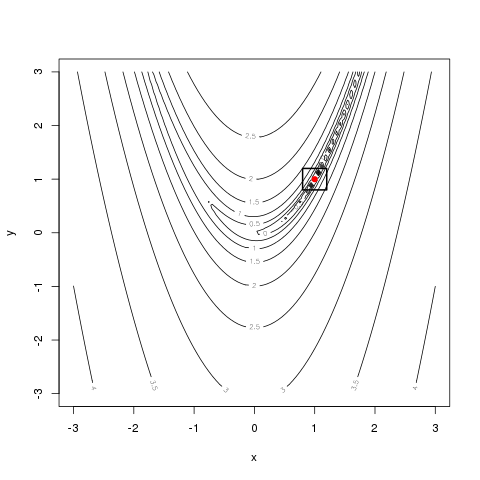
\includegraphics[scale=0.45]{a_optimization/conjugate_gradient_result.png}
\caption{Contour plot of the Rosenbrock function with the located minimum highlighted.}
\label{plot:conjugate_gradient_result}
\end{figure}

% other packages
The \texttt{gsl} package in the \texttt{multimin()} function provides an implementation of Conjugate Gradient Method that makes use of the GNU Scientific Library \cite{Hankin2011}.


% References: Deeper understanding
% The references element description includes a listing of both primary sources of information about the technique as well as useful introductory sources for novices to gain a deeper understanding of the theory and application of the technique. The description consists of hand-selected reference material including books, peer reviewed conference papers, journal articles, and potentially websites. A bullet-pointed structure is suggested.
\subsection{References}
% What are the primary sources for a technique?
% What are the suggested reference sources for learning more about a technique?

% primary sources
\subsubsection{Primary Sources}
% seminal
The Conjugate Gradient method for solving systems of linear equations was proposed by Hestenes and Stiefel in 1952 \cite{Hestenes1952}.
% optimization
Fletcher and Reeves extended the method to an optimization method for unconstrained nonlinear optimization in 1964 \cite{Fletcher1964}.

% more info
\subsubsection{More Information}
% book
Polak provides a detailed treatment of Conjugate Gradient in his text of numerical methods with suggested implementation details \cite{Polak1971} (pages 44 and 306).
Hestenes also provides a treatment of Conjugate Gradient and other numerical methods for optimization in his text \cite{Hestenes1980}.
Fletcher also wrote a book on numerical analysis for optimization with a clear treatment of Conjugate Direction Methods including Conjugate Gradient \cite{Fletcher2000} (chapter 4).
% review paper
Shewchuk provides a detailed treatment of the method and usage considerations \cite{Shewchuk1994} (page 42).
% implementation details
Press et~al.\ provide a good summary of the method with sample code in the C programming language \cite{Press2007}.

% END
\putbib\end{bibunit}
\newpage\begin{bibunit}% The Clever Algorithms Project: http://www.CleverAlgorithms.com
% (c) Copyright 2011 Jason Brownlee. Some Rights Reserved. 
% This work is licensed under a Creative Commons Attribution-Noncommercial-Share Alike 2.5 Australia License.

% Name
% The algorithm name defines the canonical name used to refer to the technique, in addition to common aliases, abbreviations, and acronyms. The name is used in terms of the heading and sub-headings of an algorithm description.
\section{BFGS Method} 
\label{sec:bfgs}
\index{Broyden-Fletcher-Goldfarb-Shanno Method}
\index{BFGS Method}
\index{Variable Metric Method}
\index{L-BFGS}
\index{Limited Memory BFGS}
\index{BFGS-B}

% other names
% What is the canonical name and common aliases for a technique?
% What are the common abbreviations and acronyms for a technique?
\emph{BFGS Method, BFGS, Broyden-Fletcher-Goldfarb-Shanno Method.}

% Taxonomy: Lineage and locality
\subsection{Taxonomy}
% To what fields of study does a technique belong?
BFGS is an optimization method for multidimensional nonlinear unconstrained functions.
% What are the closely related approaches to a technique?
BFGS belongs to the family of quasi-Newton (Variable Metric) optimization methods that make use of both first-derivative (gradient) and second-derivative (Hessian matrix) based information of the function being optimized. More specifically, it is a quasi-Newton method which means that it approximates the second-order derivative rather than compute it directly. It is related to other quasi-Newton methods such as the DFP Method, Broyden's method and the SR1 Method. 
% extensions
Two popular extension of BFGS is L-BFGS (Limited Memory BFGS) which has lower memory resource requirements and L-BFGS-B (Limited Memory Boxed BFGS) which extends L-BFGS and imposes box constraints on the method. 

% Strategy: Problem solving plan
% The strategy is an abstract description of the computational model. The strategy describes the information processing actions a technique shall take in order to achieve an objective. The strategy provides a logical separation between a computational realization (procedure) and a analogous system (metaphor). A given problem solving strategy may be realized as one of a number specific algorithms or problem solving systems. The strategy description is textual using information processing and algorithmic terminology.
\subsection{Strategy}
% What is the information processing objective of a technique?
The information processing objective of the BFGS Method is to locate the extremum of a function. 
% What is a techniques plan of action?
This is achieved by iteratively building up a good approximation of the inverse Hessian matrix.
Given an initial starting position, it prepares an approximation of the Hessian matrix (square matrix of second-order partial derivatives). It then repeats the process of computing the search direction using the approximated Hessian, computes an optimum step size using a Line Search then, updates the position, and updates the approximation of the Hessian. The method for updating the Hessian each iteration is called the BFGS rule which insures the updated matrix is positive definite.

% Heuristics: Usage guidelines
% The heuristics element describe the commonsense, best practice, and demonstrated rules for applying and configuring a parameterized algorithm. The heuristics relate to the technical details of the techniques procedure and data structures for general classes of application (neither specific implementations not specific problem instances). The heuristics are described textually, such as a series of guidelines in a bullet-point structure.
\subsection{Heuristics}
% What are the suggested configurations for a technique?
% What are the guidelines for the application of a technique to a problem instance?

\begin{itemize}
	\item It requires a function where the the functions gradient (first partial derivative) can be computed at arbitrary points.
	\item It does not require second-order derivatives as it approximates the Hessian matrix, making it less computationally expensive compared to Newton's method.
	\item It requires a relatively large memory footprint, as it maintains an $n*n$ Hessian matrix, where $n$ is the number of variables. This is a limitation on the methods scalability.
	\item The rate of convergence is superlinear and the computational cost of each iteration is $O(n^2)$ \cite{Nocedal1999}.
	\item The L-BFGS extension to BFGS is intended for functions with very large numbers of parameters ($>1000$).
	\item The stopping condition is typically a minimum change is response or a minimum gradient.
	\item BFGS is somewhat robust and self correcting in terms of the search direction and as such it does not require the use of exact line searches when determining the step size.
\end{itemize}

% sample script in R
\subsection{Code Listing}
% listing
Listing~\ref{stats_bfgs} provides a code listing of the BFGS method in R solving a two-dimensional nonlinear optimization function. Figure~\ref{plot:bfgs_result} provides a plot of the test problem with the located minimum highlighted.

% algorithm and package
The example uses the \texttt{optim()} function in the \texttt{stats} core package configured to use the BFGS method \cite{RDCT2011a}. The \texttt{optim()} function is for General-purpose Optimization, for more information on this library type: \texttt{library(help="stats")}, and for more information on the function type: \texttt{?optim}.

% problem
The test problem is the Rosenbrock function in two-dimensions where the optimum is at $x,y=1$. The starting position for the algorithm is taken as a random point $x,y \in [-3,3]$. The gradient for this function is specified and is used by the optimization method.

% TODO consider capturing algorithm progression (using par)

\lstinputlisting[firstline=7,language=r,caption={Example of BFGS in R using the \texttt{optim()} function in the \texttt{stats} core package.}, label=stats_bfgs]{../src/algorithms/optimization/stats_bfgs.R}

\begin{figure}[htp]
\centering
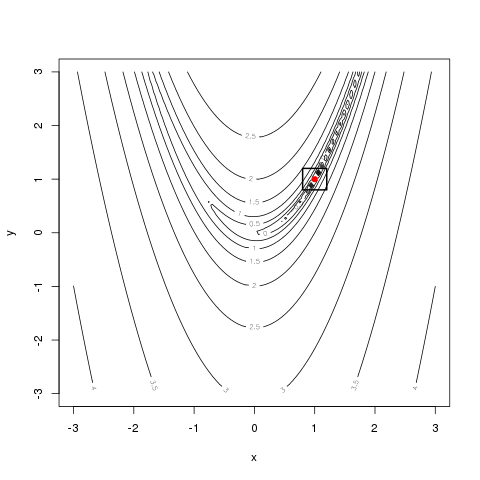
\includegraphics[scale=0.45]{a_optimization/bfgs_result.png}
\caption{Contour plot of the Rosenbrock function with the located minimum highlighted.}
\label{plot:bfgs_result}
\end{figure}

% other packages
The \texttt{optim()} function in the \texttt{stats} core package also offers an implementation of BFGS with both the Limited Memory (L-BFGS) and box constraint (BFGS-B) extensions based on the FORTRAN implementation described by Zhu et~al.\ \cite{Zhu1997}. The \texttt{gsl} package in the \texttt{multimin()} function provides an implementation of BFGS method that makes use of the GNU Scientific Library \cite{Hankin2011}.

% References: Deeper understanding
% The references element description includes a listing of both primary sources of information about the technique as well as useful introductory sources for novices to gain a deeper understanding of the theory and application of the technique. The description consists of hand-selected reference material including books, peer reviewed conference papers, journal articles, and potentially websites. A bullet-pointed structure is suggested.
\subsection{References}
% What are the primary sources for a technique?
% What are the suggested reference sources for learning more about a technique?

% primary sources
\subsubsection{Primary Sources}
% seminal 
The BFGS method was published by four authors at the same time in 1970: Broyden \cite{Broyden1970}, Fletcher \cite{Fletcher1970}, Goldfarb \cite{Goldfarb1970}, and Shanno \cite{Shanno1970}.
% extensions
The L-BFGS method was described by Nocedal \cite{Nocedal1980} and the L-BFGS-B extension was described by Byrd et~al.\ \cite{Byrd1995}.

% more info
\subsubsection{More Information}
% books
Nocedal and Wright provide a full description of the BFGS, L-BFGS and L-BFGS-B methods as well as full range of Quasi-Newton methods in their text on numerical optimization \cite{Nocedal1999}.
Press et~al.\ provide a good summary of the method with sample code in the C programming language \cite{Press2007} (Chapter 10.9).



% END
\putbib\end{bibunit}
